\chapter{BCR+: Um Novo Modelo de Redes Organizadas em Módulos} \label{cap:bcr}

% comparativo
% Número de parâmetros:
% - BCR+: 8 (6 do BCR + 2, e um deles é G)
% - LFR: 7
% - CGW: 11
%
% - BCR+ possui mais parâmetros do que o LFR, mas é mais simples pelo fato de que todas as combinações são permitidas.
%
% Crescimento:
% - BCR+ e CGW são. LFR não é.
%
% Restrição a dependências entre módulos
% - Só no BCR+ é um parâmetro, G.
%
% Combinações inválidas:
% - Apenas o LFR possui combinações de parâmetros inválidas.
%
% Semântica dos parâmetros:
% - No LFR, todos os parâmetros são propriedades das redes. No BCR+ e no CGW, propriedades como expoente da distribuição de graus e proporção de arestas externas devem ser inferidos.

\begin{section}{Introdução}

BCR é um modelo que gera redes orientadas, livres de escala e sem módulos. Assim como os modelos BA e CGW, ele utiliza os mecanismos de crescimento e ligação preferencial.

% No contexto desta pesquisa foi desenvolvido o modelo BCR+, que generaliza o modelo BCR adicionando módulos à construção da rede.
No contexto desta pesquisa foi desenvolvido um modelo baseado no BCR, chamado BCR+, que adiciona módulos à construção da rede. O modelo BCR+ foi desenvolvido por causa da dificuldade de encontrar modelos de redes organizadas orientadas em módulos nas etapas iniciais da pesquisa. O modelo apresenta uma vantagem em relação aos demais, que é a possibilidade de se restringir, através de um dos seus parâmetros ($G$), as dependências permitidas entre vértices pertencentes a módulos distintos.

Neste capítulo é apresentado o modelo BCR+. Como ele generaliza o modelo BCR, optou-se por não descrever o modelo BCR separadamente.

% \end{section}
% 
% \begin{section}{Descrição}
	O modelo BCR+ aceita os seguintes parâmetros:

	\begin{itemize}
	\item número de vértices, $n$;
	\item um grafo orientado de dependências entre módulos, $G$;
	\item três probabilidades, $p_1$, $p_2$ e $p_3$, com $p_1 + p_2 + p_3 = 1$;
	\item uma constante $\mu$, com $0 \le \mu \le 1$;
	\item grau de entrada base, $\din$;
	\item grau de saída base, $\dout$.
	\end{itemize}

	O grafo $G$ contém um vértice para cada módulo que será criado e define uma relação de dependência entre os módulos. Um módulo $M_1$ depende de um módulo $M_2$ se $G$ contém uma aresta do vértice que representa $M_1$ para o vértice que representa $M_2$. Na rede gerada, uma aresta externa de um vértice $v_1 \in M_1$ para um vértice $v_2 \in M_2$ pode ocorrer apenas se $M_1$ depende de $M_2$ no grafo $G$. %Note que $G$ pode representar uma arquitetura modular em camadas, com $M_1$ e $M_2$ formando uma camada com dois módulos.

	\begin{figure}[htbp]
		\centering
			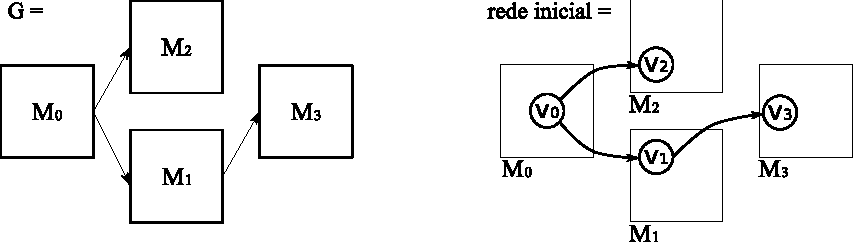
\includegraphics[scale=1]{figuras/exemplo-bcr-g}
		\caption{Rede inicial gerada a partir de um dado grafo G}
		\label{fig:bcr-g}
	\end{figure}

	O parâmetro $\mu$ controla a proporção de arestas externas na rede. Valores mais baixos levam a redes com menos arestas externas.

	O modelo BCR é um caso específico do modelo BCR+ quando $\mu = 0$ e $G$ consiste de apenas um vértice, o qual representa um único módulo. Com essa informação é fácil derivar a descrição do modelo BCR a partir da descrição do modelo BCR+ apresentada a seguir.
	
	Na rede inicial gerada pelo modelo BCR+, cada módulo contém exatamente um vértice e todas as arestas externas permitidas são adicionadas. A Figura \ref{fig:bcr-g} ilustra a geração de uma rede inicial a partir de um grafo $G$. Essa rede é então modificada de acordo com 3 regras de formação que são aplicadas sucessivamente, em ordem aleatória, até a rede alcançar o número de $n$ vértices. A cada passo do algoritmo, a probabilidade de se aplicar a regra $i$ é $p_i$.
	
\end{section}

\begin{section}{Regras de Formação}

Antes de descrever as regras do algoritmo, algumas definições são necessárias. A expressão $\mathrm{g}_{out}(x)$ designa o número de arestas com origem no vértice $x$, e $\mathrm{g}_{in}(x)$, analogamente, designa o número de arestas com destino no vértice $x$. A expressão ``escolher um vértice de acordo com f($x$)'' significa que a probabilidade de escolher um vértice $x$ é dada pela seguinte função de probabilidade:

$$
  \mathrm{P}(x) ~=~ \frac{ \mathrm{f}(x) }
  { \displaystyle\sum_{i} \mathrm{f}(i) }
$$

O denominador é apenas um fator de normalização, responsável por tornar a soma das probabilidades igual a 1.

\begin{figure}[htbp]
	\centering
		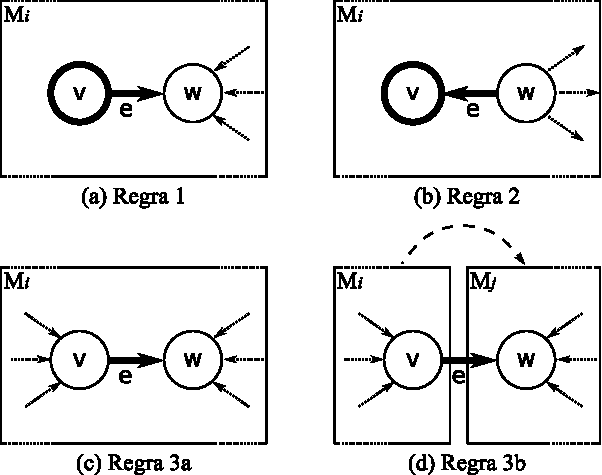
\includegraphics[scale=1]{figuras/regras-bcr}
	\caption{As regras de formação de redes do modelo BCR+. $M_i$ e $M_j$ são módulos, e $M_i$ depende de $M_j$. Os vértices e arestas criados durante a execução de cada regra estão destacados com uma linha mais grossa.}
	\label{fig:bcr-regras}
\end{figure}

As regras do modelo estão ilustradas na Figura \ref{fig:bcr-regras} e são descritas a seguir:

\begin{enumerate}

\item \emph{Adicionar um vértice com uma aresta de saída}. Um vértice existente, $w$ é escolhido de acordo com $\mathrm{f}(x) = \din + \mathrm{g}_{in}(x)$. Um novo vértice, $v$, é adicionado ao módulo que contém $w$, juntamente com uma aresta de $v$ a $w$.

\item \emph{Adicionar um vértice com uma aresta de entrada}. Um vértice existente, $w$ é escolhido de acordo com $\mathrm{f}(x) = \dout + \mathrm{g}_{out}(x)$. Um novo vértice, $v$, é adicionado ao módulo que contém $w$, juntamente com uma aresta de $w$ a $v$.

\item \emph{Adicionar uma aresta entre vértices pré-existentes}. Um vértice, $v$, é escolhido de acordo com $\mathrm{f}(x) = \dout + \mathrm{g}_{out}(x)$. Então é adicionada uma aresta do vértice $v$ a um vértice $w$, escolhido de acordo com $\mathrm{f}(x) = \din + \mathrm{g}_{in}(x)$, respeitando um dos seguintes casos:

\begin{enumerate}
  \item com probabilidade $\mu$, $w$ é escolhido dentre os vértices que estão em módulos dos quais o módulo de $v$ depende;
  \item com probabilidade $1 - \mu$, $w$ é escolhido dentre os vértices que estão no mesmo módulo que $v$.
\end{enumerate}

\end{enumerate}
\end{section}

\begin{section}{Exemplo}

A Figura \ref{fig:bcr-passo} mostra um passo da simulação do modelo BCR+, continuando a rede inicial mostrada na Figura \ref{fig:bcr-g}. Suponhamos que o parâmetro $\dout$ vale $2$ e que, neste passo da simulação, a regra 2 foi escolhida. Neste caso, é necessário escolher um vértice da rede, e essa escolha deve considerar, para cada vértice, $x$, o valor de $\mathrm{f}(x) = \dout + \gout(x)$, ilustrado na rede inicial da figura através de números entre parênteses. A probabilidade de se escolher um vértice $x$, P($x$) é, então, dada por $\mathrm{P}(x) = \frac{\mathrm{f}(x)}{\sum_i \mathrm{f}(i)}$, onde o denominador, no exemplo, é igual a 11, de forma que $\sum \mathrm{P}(x)$ = 1. A Figura \ref{fig:bcr-passo} ilustra, através de uma reta real, as probabilidades associadas à escolha cada vértice. Cada vértice ocupa, na reta, um segmento cujo tamanho é proporcional à probabilidade de ele ser escolhido. Assim, a escolha do vértice pode ser feita sorteando-se um número real entre 0 e 1 e marcando-o na reta. No exemplo, foi sorteado o número $\frac{5}{11}$, que corresponde a um ponto do segmento do vértice $v_1$ na reta. Dando seguimento à regra 2, é criado um novo vértice, $v_4$, que é atribuído ao módulo $M_1$ (o mesmo módulo ao qual pertence o vértice $v_1$), e ligado ao vértice $v_1$ através de uma aresta com origem em $v_1$.

% O vértice $v_0$ é o mais provável, com P($v_0$) = \frac{4}{11}. Os vértices $v_2$ e $v_3$, apesar de possuírem grau de saída igual a zero, têm chances de serem escolhidos, graças ao fato de que $\dout > 0$. 

\begin{figure}[htbp]
	\centering
		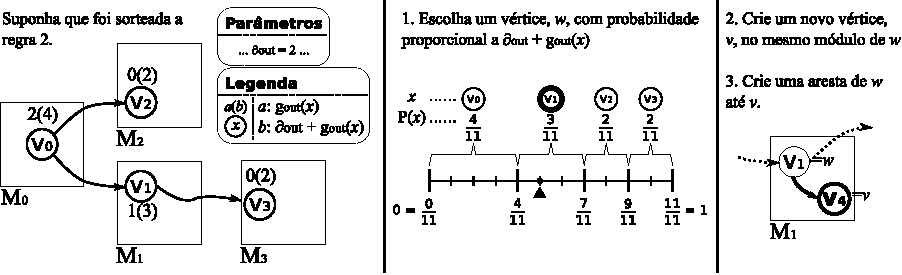
\includegraphics[scale=1]{figuras/bcr-passo}
	\caption{Um passo da simulação do modelo BCR+.}
	\label{fig:bcr-passo}
\end{figure}

Nota-se que vértices com grau de saída alto têm mais chance de ser a origem de novas arestas. O parâmetro $\dout$ reduz essa tendência fornecendo um grau de entrada base que é aplicado a todos os vértices no cálculo das probabilidades. No exemplo da Figura \ref{fig:bcr-passo}, se $\dout$ fosse igual a zero, os vértices $v_2$ e $v_3$ teriam chance nula na escolha, uma vez que o grau de saída de ambos é igual a zero. O mesmo raciocínio se aplica a $\din$ com relação ao grau de entrada.

% Considere dois vértices, $v_1$, com grau de entrada 4, e $v_2$, com grau de entrada 8. Se $\din = 0$, $v_2$ tem o dobro de chance de ser o destino de uma nova aresta; se, por outro lado, $\din = 4$, $v_2$ tem apenas $\frac{3}{2}$ de chance de receber a aresta. O mesmo raciocínio se aplica a $\dout$ com relação ao grau de saída.

 % é o uso de uma rede gerada pelo modelo como parâmetro $G$ do próprio modelo. Em termos operacionais, o modelo é executado uma vez para gerar uma rede no qual os módulos representam módulos de software e os vértices representam classes, e então é executado na segunda vez considerando a rede gerada na primeira etapa como o parâmetro $G$. Na rede resultante, os módulos seriam interpretados como classes e os vértices poderiam ser interpretados como membros das classes. As duas redes, combinadas, formariam uma rede hierárquica com três níveis: módulos, classes e membros.

% TODO: Figura

\end{section}

\begin{section}{Conclusão}
	
	O modelo BCR+, baseado no modelo BCR, gera redes livres de escala organizadas em módulos. Em relação a modelos similares, o modelo BCR+ tem a vantagem de oferecer controle sobre as dependências que podem ser geradas entre entidades que pertencem a módulos distintos. Tal possibilidade contribui para que o modelo BCR+ reproduza melhor o processo de construção de sistemas de software que se baseiam na implementação de uma arquitetura pré-definida.
	
\end{section}